\documentclass{beamer} 
\usetheme{Singapore} 

\setbeameroption{show notes}

\usepackage{color}
\usepackage{amsmath}


\title{Bayesian Inference for Arts Majors}
\author{Marius Cobzarenco}
\date{December 2012}

\begin{document}
	\maketitle
	\begin{frame}

		\frametitle{Two Schools of Thought}
		\begin{itemize}
			\item What is probability?
			\pause
			\item People have an innate understanding of uncertainty
			\pause
			\item E.g. natural languages make it easy to describe and assign likelihoods to different outcomes of a situation.
			\pause
			\item However, formalizing this intuition into maths turns out to be a bit tricky.
			\pause
			\item Consider two questions:
			\begin{enumerate}
				\item What's the probability of getting heads if you flip a coin?
				\pause
				\item What's the probability that alien life exists in the universe?
			\end{enumerate}
			\pause
			\item Historically, this distinction has lead to two opposing philosophical views of probability.
		\end{itemize}

	\end{frame}
	\note {
	\begin{itemize}
		\item The obligatory over-used stats metaphor
		\item The question "What's the probability of getting heads if a flip a coin?" is not so different as it is possible to calculate the outcome.
\item Well, maybe we can flip coins for long enough and average the results and thus probability = \emph{long term average}.
	\end{itemize}
	}

	\begin{frame}
		\frametitle{Frequentist Probability}
		\begin{columns}
			\begin{column}{0.4\textwidth}
				\begin{figure}
					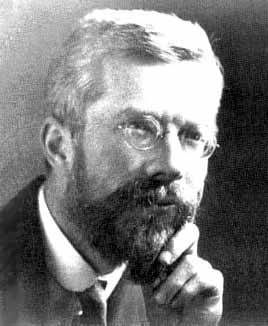
\includegraphics[scale=0.53]{fischer.jpg}
					\begin{centering}
						\small Ronald Fisher (1890 -- 1962)
					\end{centering}
				\end{figure}
			\end{column}	

			\begin{column}{0.6\textwidth}
				\begin{itemize}
					\item Probability = long term average over (hypothetical) repeated experiments.
					\pause
					\item Data is random
					\pause
					\item Quantities of interest (i.e. the parameters)  are not random, only unknown.
					\pause
					\item The sampling distribution is central.
					\pause
					\item "Standard" interpretation of probability.
				\end{itemize}
			\end{column}
		\end{columns}
	\end{frame}
	\note {
	\begin{itemize}
		\item the idea of repeated experiments is central (hence the name "freqentist")
		\item central concept: The sampling distribution of a statistic is the distribution of that statistic, considered as a random variable, when derived from a random sample of size n. 
		\item The sampling distribution depends on the underlying distribution of the population, the statistic being considered, the sampling procedure employed and the sample size used. There is often considerable interest in whether the sampling distribution can be approximated by an asymptotic distribution, which corresponds to the limiting case as n → ∞.

	\end{itemize}
	}

	\begin{frame}
		\frametitle{Bayesian Probability}
		\begin{columns}
			\begin{column}{0.4\textwidth}
					\begin{figure}
					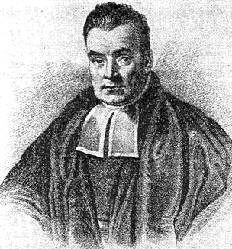
\includegraphics[scale=0.53]{bayes.jpg}
					\begin{centering}
						{\small Thomas Bayes (1701 -- 1761)}
					\end{centering}
				\end{figure}
			\end{column}	

	\begin{column}{0.6\textwidth}
		\begin{itemize}
			\item Probability = strength of belief
			\item 
 		\end{itemize}
  \end{column}
\end{columns}
		\pause
		\vspace{0.1in}
		We will be Bayesian for the rest of the presentation.
	\end{frame}

	\note {
	\begin{itemize}
		\item "subjective" probability
		\item 

	\end{itemize}
	}

	\begin{frame}
		\frametitle{Bayesian Probability}
		\begin{columns}
			\begin{column}{0.5\textwidth}
				\begin{figure}
					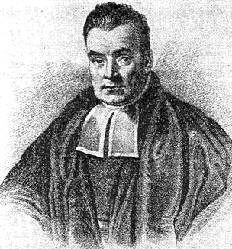
\includegraphics[scale=0.53]{bayes.jpg}
					\begin{centering}
						{\tiny Thomas Bayes (1701 -- 1761)} 
					\end{centering}
				\end{figure}
			\end{column}	
			\begin{column}{0.5\textwidth}
				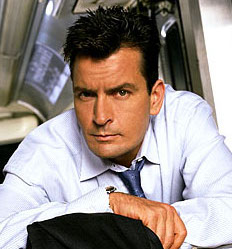
\includegraphics[scale=2.2]{newbayes.jpg}
			\end{column}	
\end{columns}
		\vspace{0.1in}
		Also... Bayes is back

	\end{frame}

	\begin{frame}
		\frametitle{Bayes Theorem}
		\begin{itemize}
			\item A bit of notation: $P(A|B)$ reads "the probability of A given B" 
			\pause
			\item E.g. the probability of being ill given that my doctor told me so
			\pause
			\item Or closer to finance, e.g.: the probability of making a profit if I put all my money on red
			\pause
			\item Bayes Theorem:
			\begin{displaymath}
			P(A|B) = \frac{P(B|A)P(A)}{P(B)}
			\end{displaymath}
			\pause
			\item The workhorse of Bayesian inference, used to compute P(what I care about | what I have observed).
			\pause
			\item It also fits on a t-shirt
		\end{itemize}
	
	\end{frame}

	\note {
		\begin{itemize}
			\item e.g. the probability of being ill given that my doctor told me so
			\item or for an example closer to finance: the probability of making a profit if I put all my money on red
			\item If you need ideas for Chirstmas presents
		\end{itemize}
	}

	\begin{frame}


	\end{frame}


% \input{hitrate.tex}

\end{document}